% Based on template from the "IILC Dissertation Style"
% https://www.illc.uva.nl/PhDProgramme/current-candidates/other/illcdiss.html#latex

\thispagestyle{empty}
% change page style for pages before actual content
{\pagestyle{empty} 

% Empty page after the initial title page
%\mbox{}\newpage
%\setcounter{page}{1}

% with memoir:
\clearpage % end title page
\null
\newpage

% Page 1: the half-title / `franse pagina'
\vspace*{2cm}
\begin{center}
\Huge\textbf{Neuroplasticity of Attention} % CHANGE THIS TO MATCH THESIS TITLE
\end{center}

%% Page 2: Colophon
\clearpage
\vspace*{\fill}
\begingroup % to change formatting only temporarily
\small
\setlength{\parskip}{\baselineskip} % add space between paragraphs
\setlength\parindent{0pt} % no indents
The investigations in this thesis were supported by 
a Research Talent Grant (452-10-018)  % CHANGE grant   
from 
the Netherlands Organization for Scientific Research (NWO). % CHANGE funding body


\includegraphics{_bookdown_files/FSC.pdf} \newline
This thesis was typeset using \LaTeX\ and the \verb+bookdown+ R-package \newline
ISBN: xxx-xx-xxx-xxxx-x \newline % CHANGE ISBN
Printing: Ridderprint BV \newline % CHANGE printer
Cover art: X, \url{www.website.com} % CHANGE cover art credits

\includegraphics{_bookdown_files/CC-BY.eps} \newline
An online version of this thesis is available at 
\url{lcreteig.github.io/thesis} % CHANGE thesis website
, licensed under a 
Creative Commons Attribution 4.0 International License. % CHANGE license
\endgroup
\begin{center}
\Huge\textbf{Neuroplasticity of Attention} % CHANGE THIS TO MATCH THESIS TITLE
\par\vspace {1cm}
\Large\textit{How brain stimulation and mental fatigue\\
affect attentional performance} % CHANGE THIS TO MATCH SUBTITLE
\par\vspace {4cm}
{\large \sc Academisch Proefschrift}
\par\vspace {1cm}
\linespread{1.3}{\normalsize ter verkrijging van de graad van doctor\\
aan de Universiteit van Amsterdam\\
op gezag van de Rector Magnificus\\
prof. dr. ir. K.I.J. Maex\\ % CHECK IF THIS MATCHES CURRENT RECTOR MAGNIFICUS
ten overstaan van een door het College voor Promoties ingestelde commissie,\\
\mbox{in het openbaar te verdedigen in de Agnietenkapel}\\  %CHANGE
% The part after "de" should either read "Agnietenkapel" or "Aula der Universiteit"
%op [……]dag […datum…] […maand…] 20[….], te [……] uur \\ } %CHANGE
op woensdag 20 november 2019, te 14.00 uur \\ } %CHANGE
% e.g. maandag 1 januari 2001, te 12.00 uur
\par\vspace {1cm} {door}
\par \vspace {1cm} 
{Leon Cyro Reteig} % CHANGE TO YOUR FULL NAME 
\par\vspace {1cm} % and your birthplace
{geboren te Amsterdam} %CHANGE
% If your country of birth is the Netherlands, this should be only your place of birth,
% e.g.: geboren te Amsterdam
% If you were born outside the Netherlands, you should add your country of birth,
% e.g.: geboren te San Francisco, Verenigde Staten van Amerika
\end{center}

%% Page 4: info on thesis committee
\clearpage
\noindent%
{\bf Promotiecommissie:}\\
\\
\begin{tabular}[t]{@{}p{2.75cm}ll}
Promotores:    & prof. dr. K.R. Ridderinkhof    & Universiteit van Amsterdam \\  %CHANGE
               & prof. dr. H.A. Slagter         & Universiteit van Amsterdam \\  %CHANGE
\\
% Uncomment the two lines below if there are copromotor(es)
%Copromotor(es): & prof. dr. something something  & Universiteit van Amsterdam \\  %CHANGE
%\\
Overige leden: & prof. dr. M.M. Lorist          & Rijksuniversiteit Groningen \\ %CHANGE
               & prof. dr. B.U. Forstmann       & Universiteit van Amsterdam \\  %CHANGE
               & prof. dr. H.M. Huizenga        & Universiteit van Amsterdam \\  %CHANGE
               & prof. dr. V.A.F. Lamme         & Universiteit van Amsterdam \\  %CHANGE
               & dr. I.G. Sligte                & Universiteit van Amsterdam \\  %CHANGE
               & dr. W.P.M. van den Wildenberg  & Universiteit van Amsterdam \\  %CHANGE
\\               
\end{tabular}\\

\noindent%
\begin{tabular}[t]{@{}p{2.75cm}l}
Faculteit:     & Faculteit der Maatschappij- en Gedragswetenschappen \\ %CHANGE
\end{tabular}\\

%% Page 5: quotes

% poem attribution (from memoir class manual, chapter on poetry)
\newcommand{\attrib}[1]{%
  \nopagebreak{\raggedleft\footnotesize #1\par}}
% dotted line for omitted stanzas in poem (http://xpt.sourceforge.net/techdocs/language/latex/latex03-LaTexUsage/ar01s18.html)
\newcommand{\dotrule}[1]{%
   \parbox[t]{#1}{\dotfill}}

\clearpage
\begin{vplace} % center vertically

% EPIGRAPH
\setlength\epigraphwidth{0.5\textwidth}
\epigraph{There's an awful lot of talk about groundbreaking research\ldots\ [G]roundbreaking is what you do when you start a building. You go into a field and you dig a hole in the ground. If you're only rewarded for groundbreaking research, there's going to be a lot of fields with a small hole in, and no buildings.}{\textsc{Ottoline Leyser}\\ \textit{The Life Scientific, BBC Radio 4}}

\vspace{2\baselineskip}

% POEM
\PoemTitle*{O ME! O LIFE!}
\settowidth{\versewidth}{Of myself forever reproaching myself, (for who more foolish than)} % length of longest line
\begin{verse}[\versewidth]
O \textsc{me} ! O life ! of the questions of these recurring, \\
\dotrule{\versewidth} \\
Of myself forever reproaching myself, (for who more foolish than \\> I, and who more faithless?) \\
\dotrule{\versewidth} \\
Of the poor results of all, of the plodding and sordid crowds I \\> see around me, \\
Of the empty and useless years of the rest, with the rest me inter- \\> twined, \\
The question, O me ! so sad, recurring--- What good amid these, \\> O me, O life? \\
\vinphantom{The question, O me ! so sad, } \textbf{\textit{\footnotesize Answer.}} \\
\dotrule{\versewidth} \\
That the powerful play goes on, and you may contribute a verse.\\
\end{verse}
\attrib{(1, 3, 5--8, 10)}
\attrib{---Walt Whitman}

\end{vplace}

} % End \pagestyle{empty}
\clearpage